\subsection{A Quick Overview of Parallel Software}
\makesubcontentsslidessec

\begin{frame}{``Native'' Programming Models and Tools}
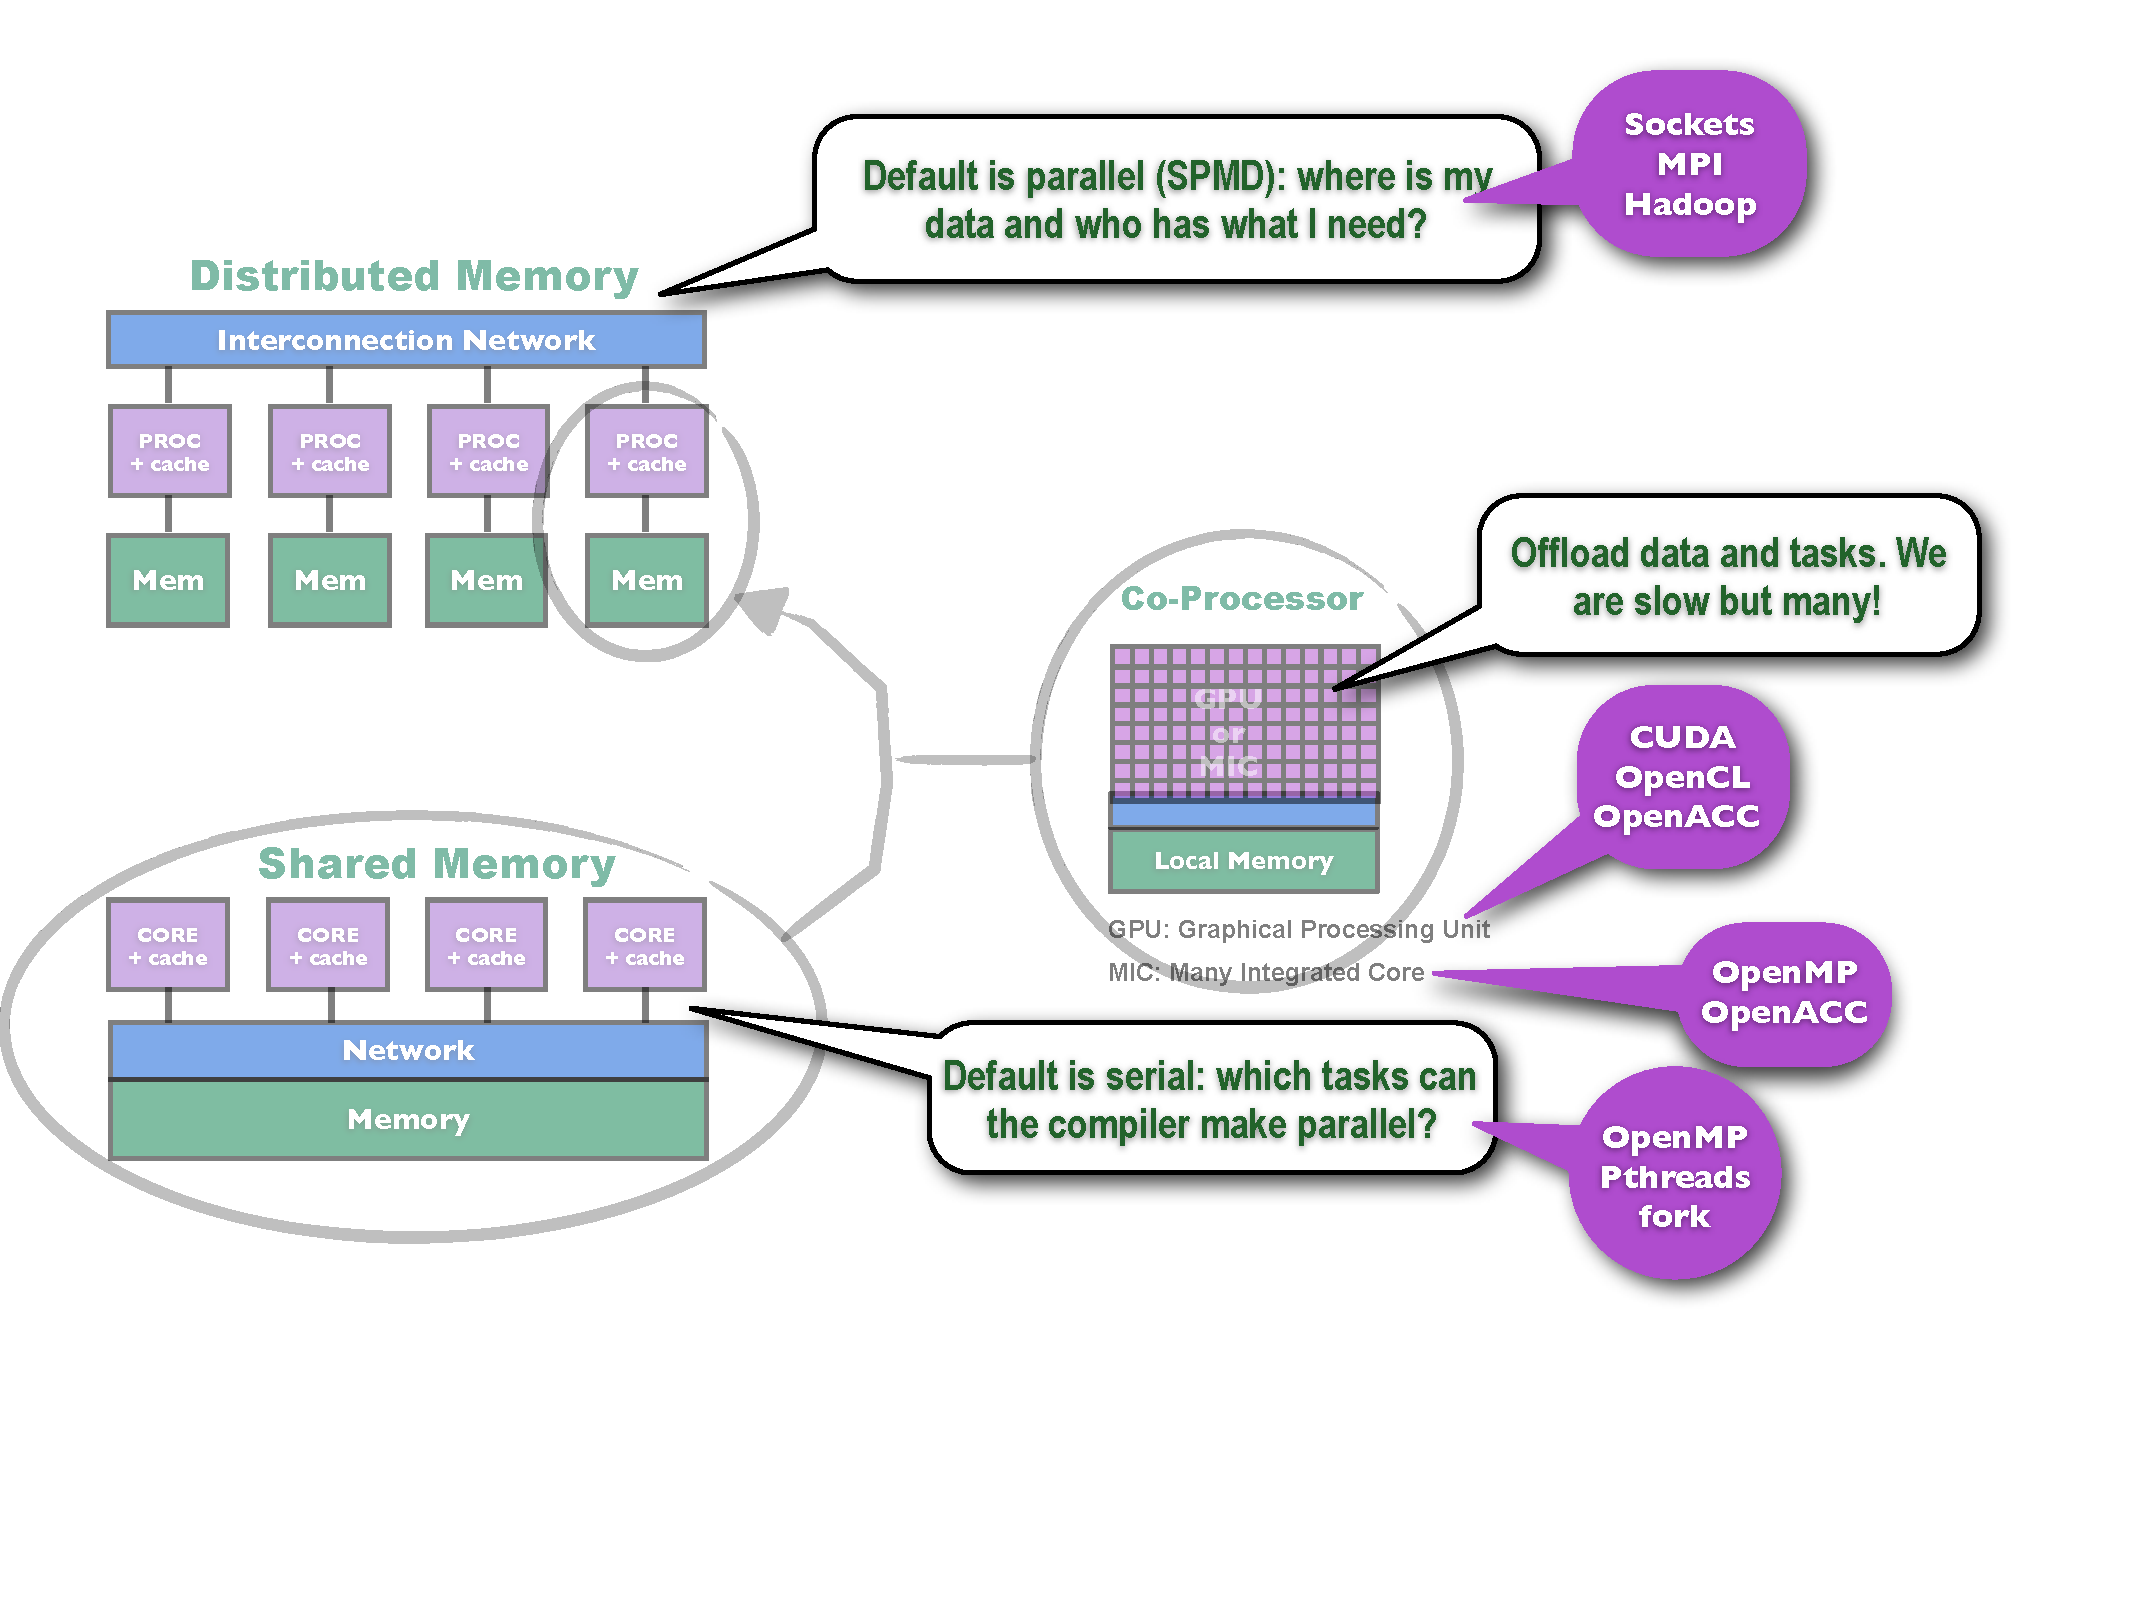
\includegraphics[width=0.95\textwidth]
{../common/pics/hardware/ParallelHardware6.pdf}
\end{frame}

\begin{frame}{Distributed Programming Works in Shared Memory}
\includegraphics[width=0.95\textwidth]
{../common/pics/hardware/ParallelHardware29.pdf}
\end{frame}

\begin{frame}{R Interfaces to Low-Level Native Tools}
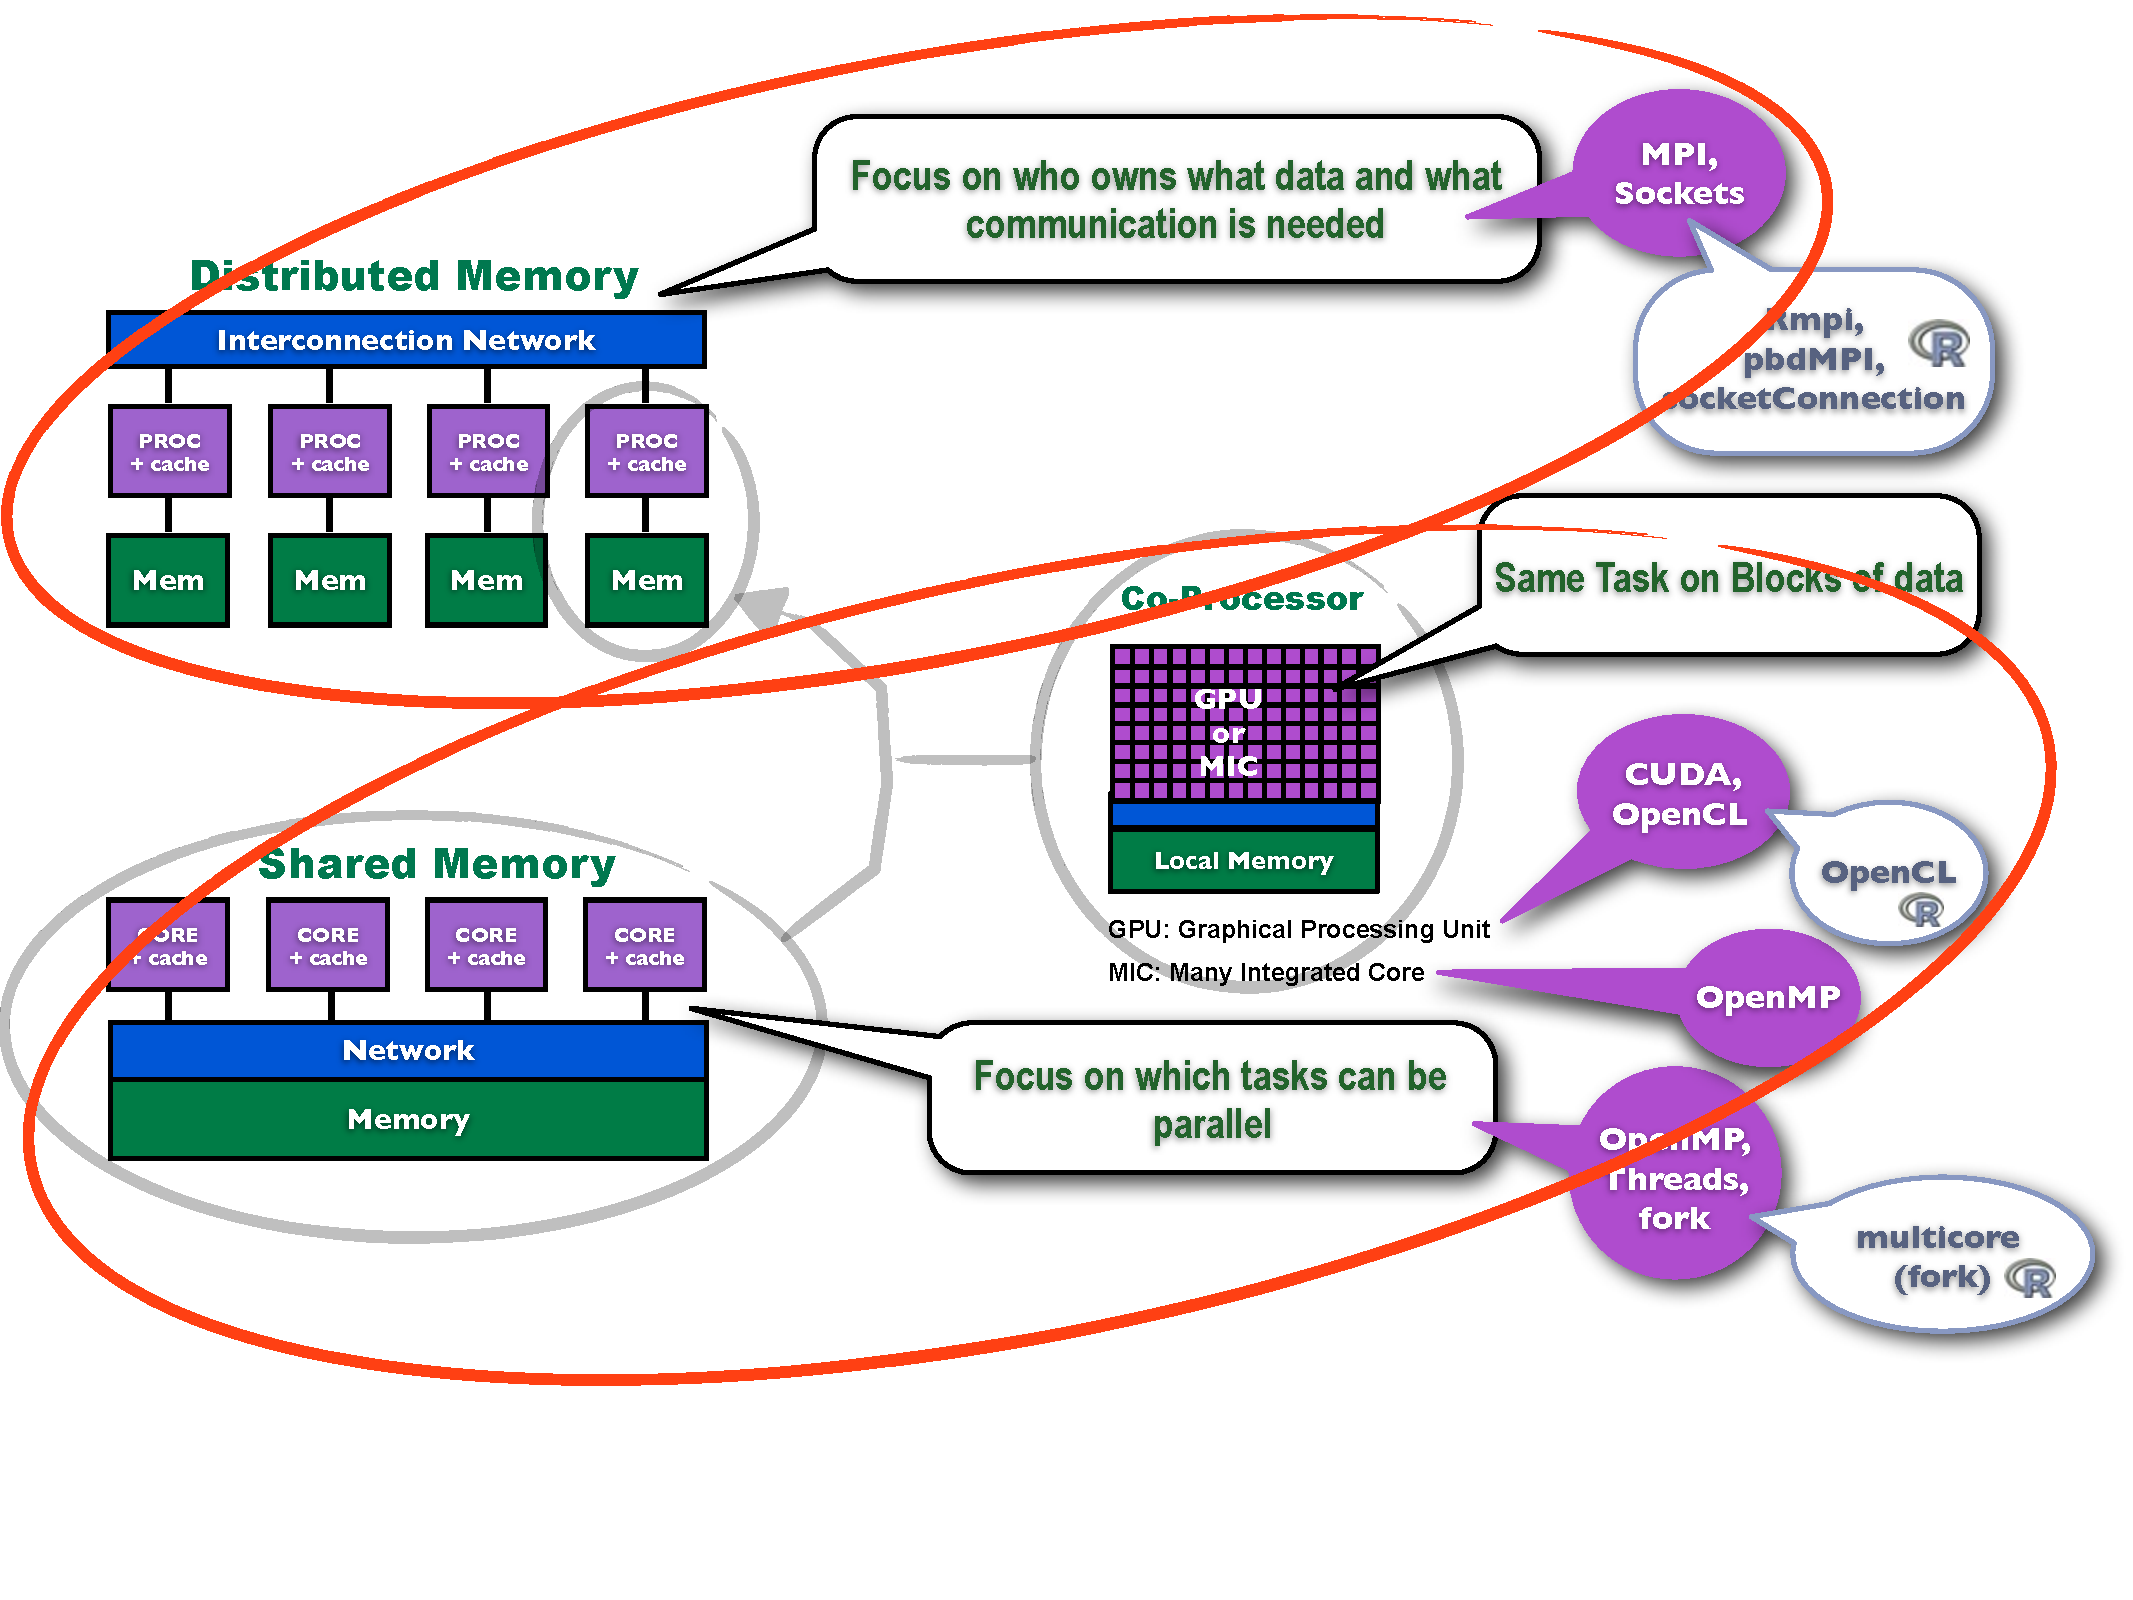
\includegraphics[width=0.95\textwidth]
{../common/pics/hardware/ParallelHardware10.pdf}
\end{frame}

\begin{frame}{R and \pbdR Interfaces to HPC Libraries}
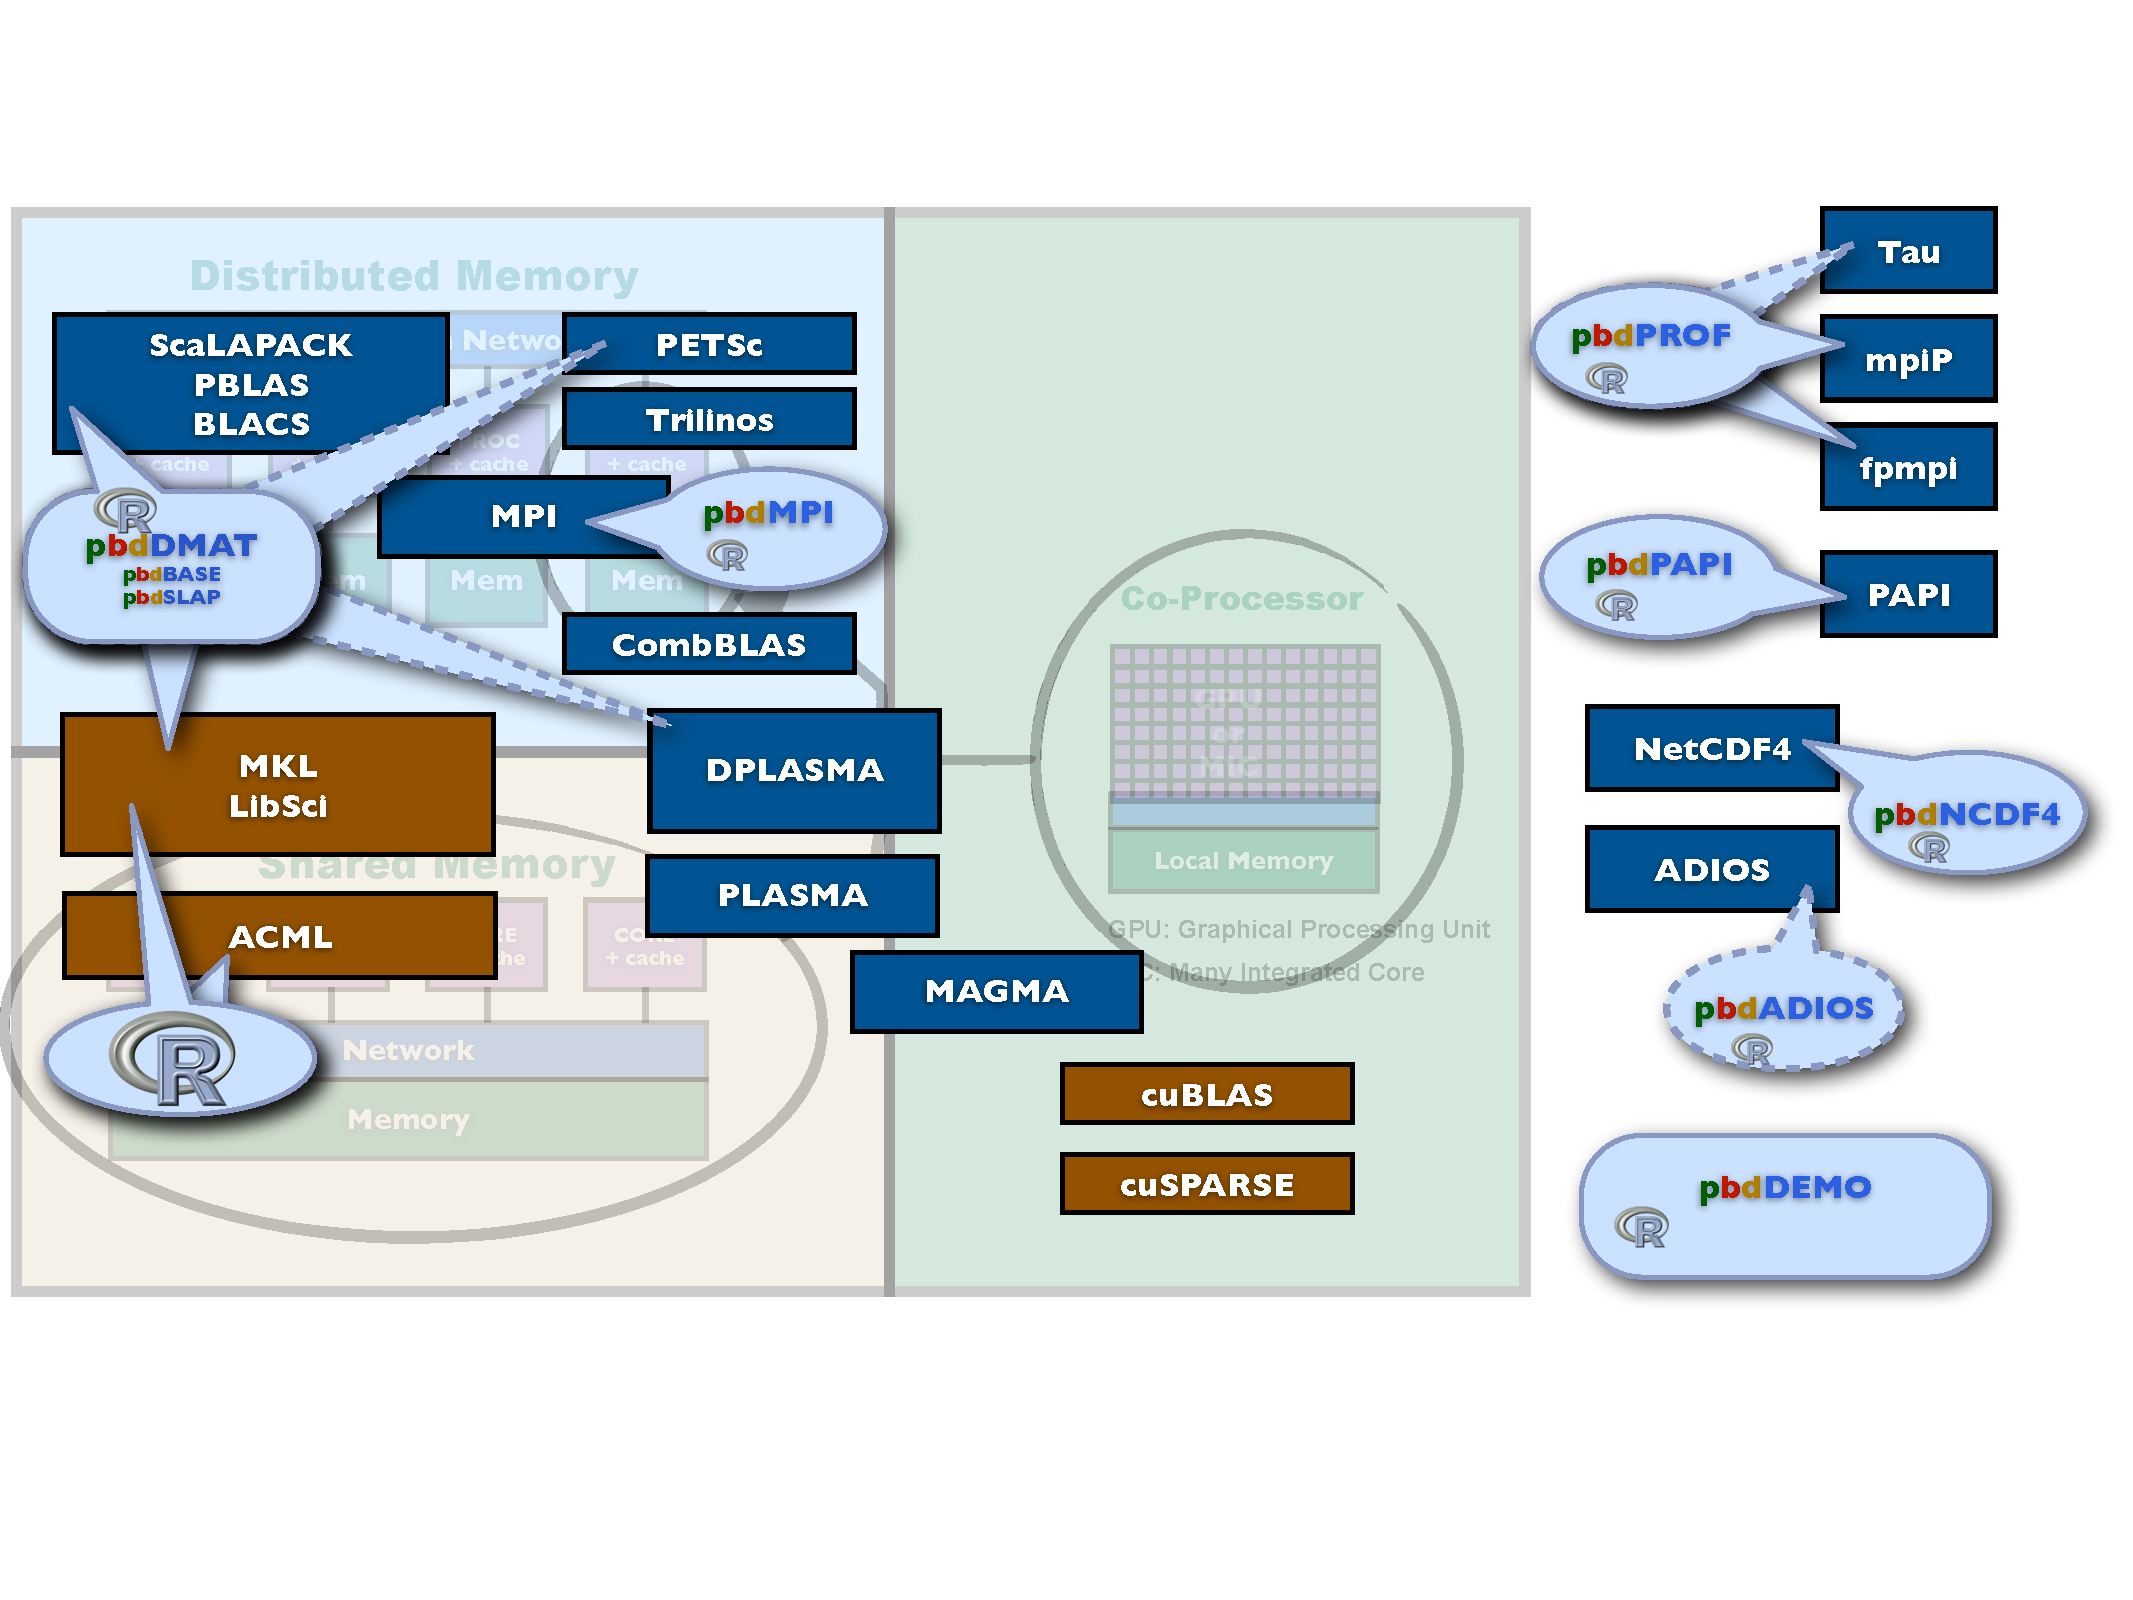
\includegraphics[height=\textheight]
{../common/pics/hardware/ParallelHardware27.pdf}
\end{frame}

